%----------------------------------------------------------------------------------------
%    PACKAGES AND THEMES
%----------------------------------------------------------------------------------------

\documentclass[aspectratio=169,xcolor=dvipsnames]{beamer}
\usetheme{SimpleDarkBlue}
\usepackage[UTF8]{ctex}
\usepackage{hyperref}
\usepackage{graphicx} % Allows including images
\usepackage{booktabs} % Allows the use of \toprule, \midrule and \bottomrule in tables
\usepackage[backend=bibtex,sorting=none]{biblatex}
\addbibresource{Pre.-Empathy-in-VR/reference.bib} %BibTeX数据文件及位置
\setbeamerfont{footnote}{size=\tiny}
%----------------------------------------------------------------------------------------
%    TITLE PAGE
%----------------------------------------------------------------------------------------

\title{Empathy in VR}

\author{The Sixth Group}

\date{\today} % Date, can be changed to a custom date

%----------------------------------------------------------------------------------------
%    PRESENTATION SLIDES
%----------------------------------------------------------------------------------------

\begin{document}

\begin{frame}
    \titlepage
\end{frame}

\begin{frame}{Overview}
    \tableofcontents
\end{frame}

% First Teammate
\section{Background}

% Second Teammate
\section{Technology}

% Third Teammate
\section{应用}
\begin{frame}{应用}
    \begin{center}
        \Large{虚拟现实中的移情应用}\\
        \vspace{0.5cm}
        \normalsize{71122227朱瑾贤}
        \\
        \vspace{0.5cm}
        \normalsize{角色:应用专家}
    \end{center}
\end{frame}

\begin{frame}{应用}
    \begin{columns}[c]    
        \column{0.5\textwidth}
        \begin{center}
            \textbf{\large 专业培训} \\
            \vspace{0.1cm}
            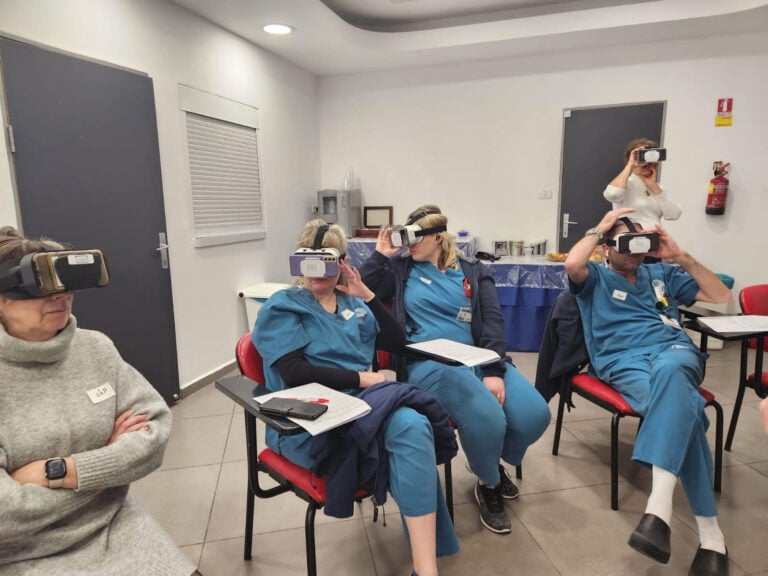
\includegraphics[height=2.8cm]{Pre.-Empathy-in-VR/section3_picture/doctortraining.jpg} \\
            \vspace{0.1cm}
            \begin{minipage}{0.95\textwidth}
                \centering\small
                提升医疗服务提供者、教师和其他专业人士的移情能力,以改善服务质量
            \end{minipage}
        \end{center}
        
        \column{0.5\textwidth}
        \begin{center}
            \textbf{\large 教育应用} \\
            \vspace{0.1cm}
            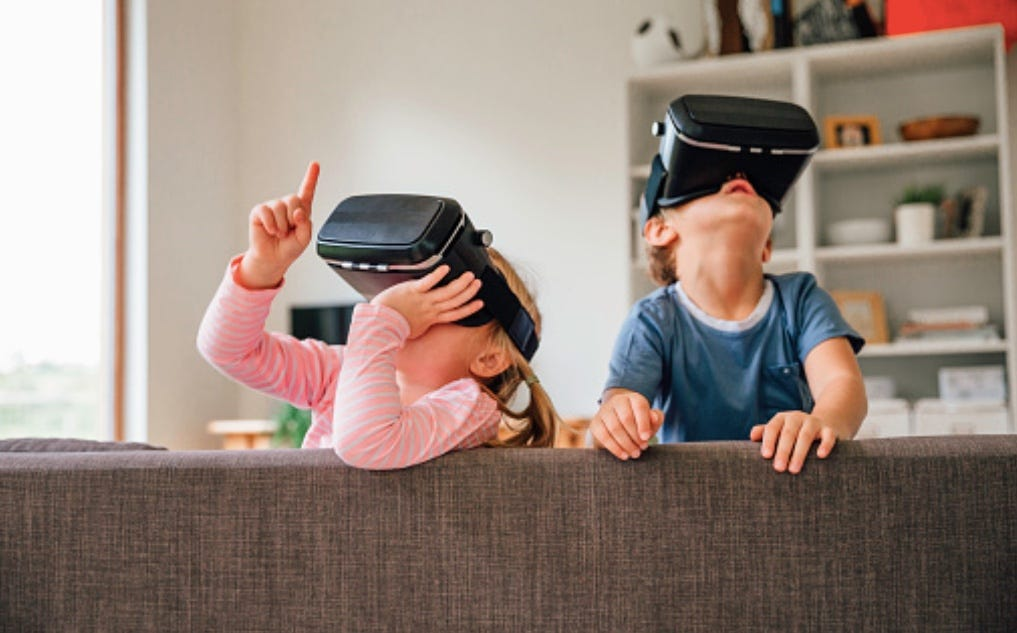
\includegraphics[height=2.8cm]{Pre.-Empathy-in-VR/section3_picture/childrenempathy1.jpg} \\
            \vspace{0.1cm}
            \begin{minipage}{0.95\textwidth}
                \centering\small
                为儿童和公众提供移情教育,促进社会包容和多元理解
            \end{minipage}
        \end{center}
    \end{columns}
    
    \begin{block}{应用进展}
        虚拟现实移情应用正在从概念验证过渡到实际实施阶段,主要通过专业培训和公共教育推进移情能力的发展。
\end{block}
\end{frame}

\begin{frame}{虚拟现实移情在专业培训中的应用:以医学培训为例}
    \begin{columns}[T]
        \begin{column}{0.45\textwidth}
            \vbox to 6cm{
                \vfill
                \centering
                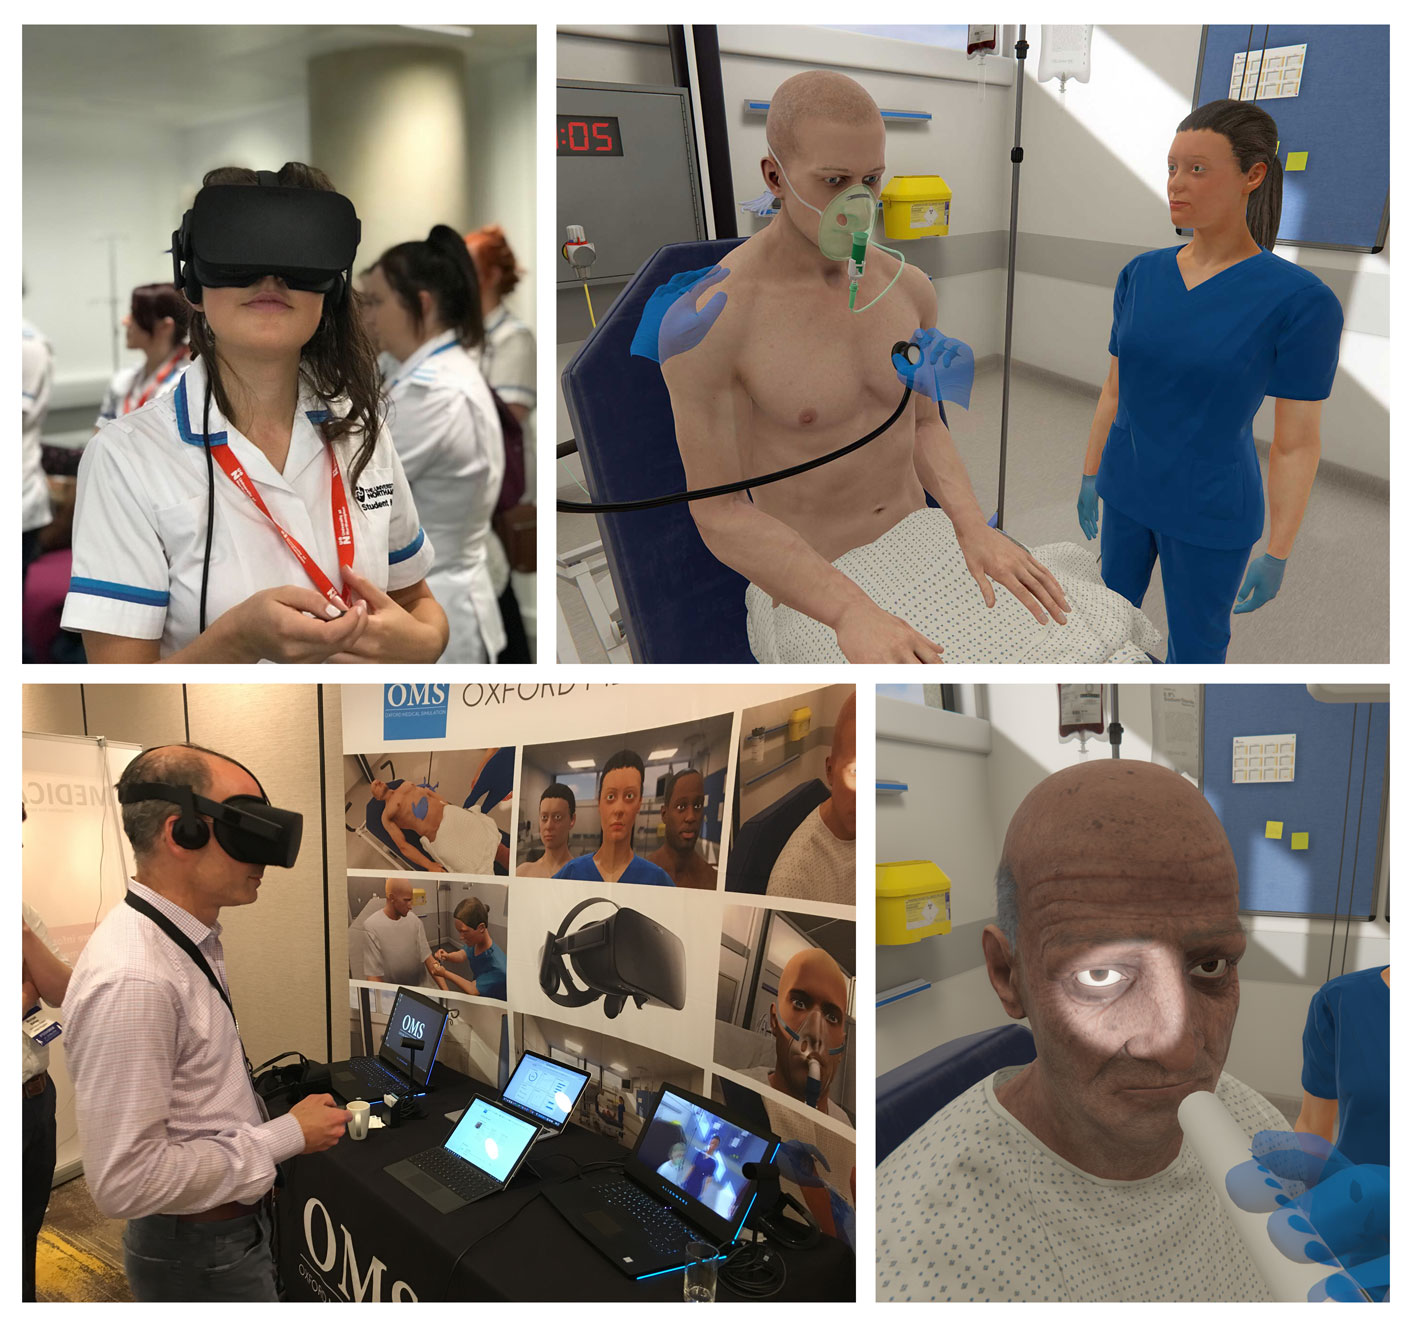
\includegraphics[height=6cm]{Pre.-Empathy-in-VR/section3_picture/medical_training.jpg}
                \vfill
            }
        \end{column}
        
        \begin{column}{0.55\textwidth}
            \vbox to 6cm{
                \vfill
                \begin{block}{虚拟现实移情应用在医学培训:背景}
                
                    研究表明医学生在教育过程中的同理心水平往往会下降,这使得在医学培训中有效实践同理心技能变得尤为重要。\footfullcite{kleinsmith2015understanding}
                    
                    在医学教育中,同理心主要被视为认知过程,即理解他人的关切,而非感受他人的痛苦。传统上,同理心训练通常通过与其他学生角色扮演或与标准化患者(SPs)互动来进行,但这些方法需要大量资源和时间安排。因此,虚拟患者作为一种补充训练方式具有潜在价值。
                \end{block}
                \vfill
            }
        \end{column}
    \end{columns}
\end{frame}

\begin{frame}{虚拟现实移情在专业培训中的应用:研究方法}
    \begin{columns}[T]
        \begin{column}{0.45\textwidth}
            \vbox to 6cm{
                \vfill
                \centering
                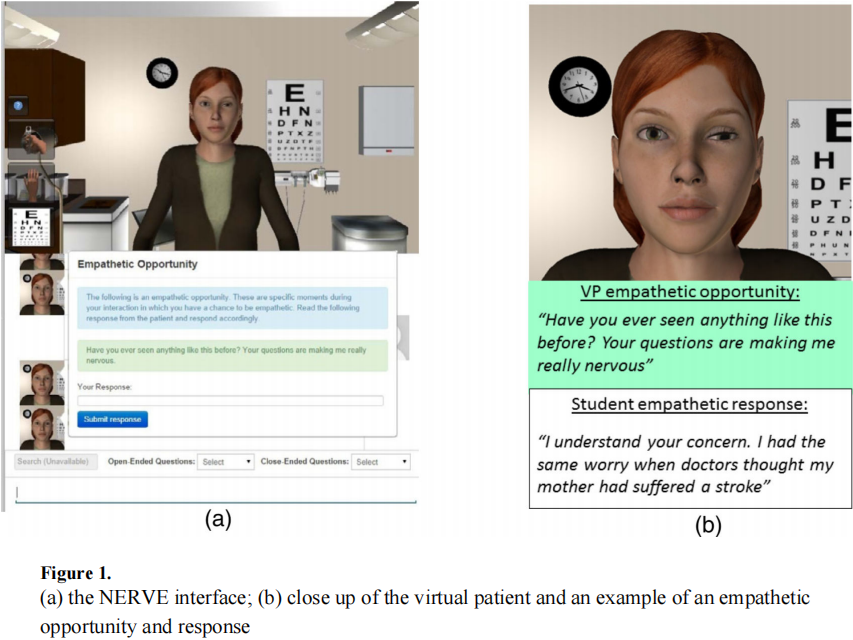
\includegraphics[height=5cm]{Pre.-Empathy-in-VR/section3_picture/medicalvr.png}
                \vfill
            }
        \end{column}
        
        \begin{column}{0.55\textwidth}
            \vbox to 6cm{
                \vfill
                \begin{block}{实验设计与评估方法}
                    研究者设计了一项对比实验,让三年级医学生在两种环境中进行互动:
                    \begin{itemize}
                        \item 使用NERVE(神经学检查演练虚拟环境)系统与虚拟患者互动
                        \item 在医院神经科部门的检查室与标准化患者互动
                    \end{itemize}
                    
                    两种患者均提出相同的同理心机会,例如:"医生,这看起来严重吗?我很担心"
                    
                    学生的回应被记录并由外部评估者使用"同理心沟通编码系统"(ECCS)进行评分分析
                \end{block}
                \vfill
            }
        \end{column}
    \end{columns}
\end{frame}

\begin{frame}{虚拟现实移情在专业培训中的应用:研究结果}
    \begin{columns}[T]
        \begin{column}{0.45\textwidth}
            \vbox to 6cm{
                \vfill
                \centering
                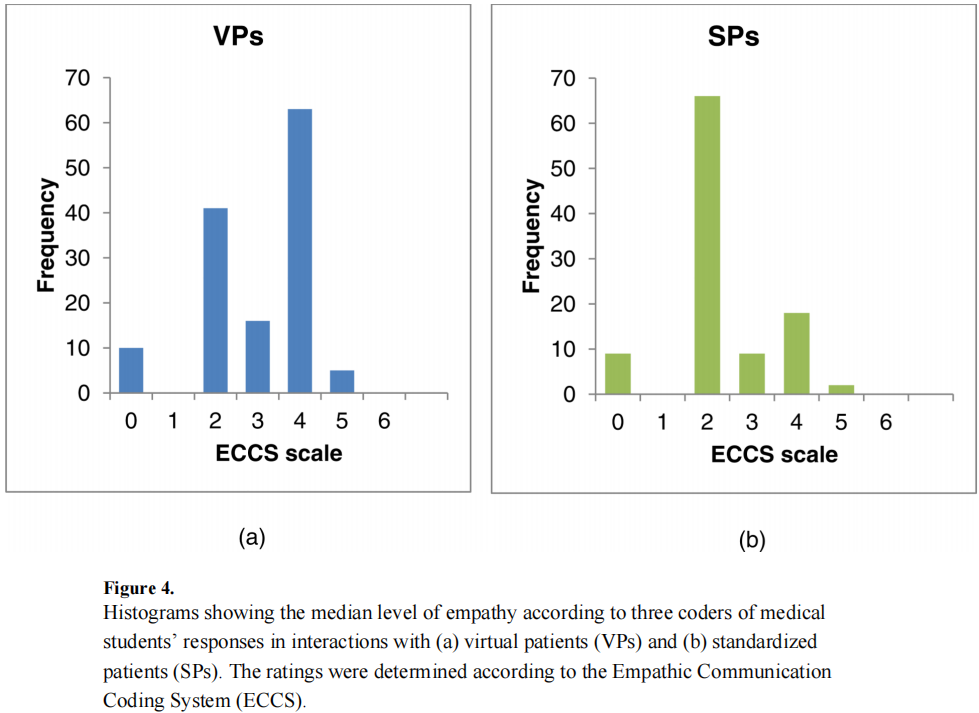
\includegraphics[height=4.8cm]{Pre.-Empathy-in-VR/section3_picture/medicalresult.png}
                \vfill
            }
        \end{column}
        
        \begin{column}{0.55\textwidth}
            \vbox to 6cm{
                \vfill
                \begin{block}{主要研究结果}
                    \textbf{虚拟患者训练效果显著优于标准化患者}:
                    \begin{itemize}
                        \item 同理心评分中位数:虚拟患者4分,标准化患者2分
                        \item 回应长度与同理心水平呈显著正相关(p<0.05)
                        \item 虽然虚拟患者被认为"人工"或"不真实",但这种人工性在早期医学教育中成为优势
                    \end{itemize}
                    
                    \textbf{实证研究证明}:
                    学生在虚拟环境中可以花更多时间思考适当回应,在没有被评判压力下练习,并且能够更好地识别同理心机会,这有助于提高未来与真实患者互动的同理心水平。
                \end{block}
                \vfill
            }
        \end{column}
    \end{columns}
\end{frame}

\begin{frame}{虚拟现实移情在儿童教育中的应用:同理心游戏框架设计}
    % 上部分放图片
    \vbox to 0.27\textheight{
        \vfill
        \centering
        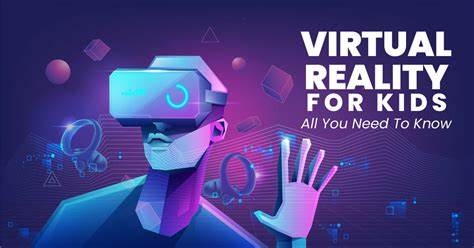
\includegraphics[height=0.35\textheight]{Pre.-Empathy-in-VR/section3_picture/childbg.jpg}
        \vfill
    }
    
    % 下部分放文字
    \vbox to 0.73\textheight{
        \vfill
        \begin{block}{虚拟现实移情应用在儿童教育:背景}
             研究表明儿童的同理心需要有意识地培养和促进,特别是在6-9岁这个关键年龄段,孩子们开始将注意力从自身转向周围的人。
            传统角色扮演活动在发达国家中的减少,与技术使用的增加有关。同时,游戏设计和虚拟现实研究者认为VR技术具有极大潜力来支持儿童的同理心发展。
                
            该研究旨在设计一个虚拟现实同理心游戏框架,探索如何利用VR技术为儿童创造有效的同理心体验。\footfullcite{muravevskaia2023designing}   
        \end{block}
        \vfill
    }
\end{frame}

\begin{frame}{虚拟现实移情在儿童教育中的应用:研究方法}
    \begin{columns}[T]
        \begin{column}{0.45\textwidth}
            \vbox to 6cm{
                \vfill
                \centering
                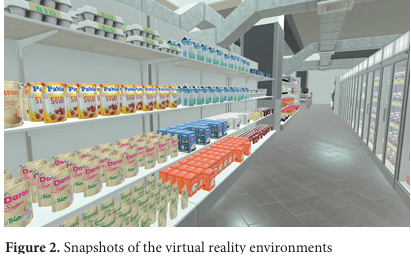
\includegraphics[height=4.3cm]{Pre.-Empathy-in-VR/section3_picture/childexperiment.png}
                \vfill
            }
        \end{column}
        
        \begin{column}{0.55\textwidth}
            \vbox to 6cm{
                \vspace{-0.5cm} % 添加负空间向上移动内容
                \begin{block}{实验设计与评估方法}
                    研究分为三个主要阶段:
                \begin{itemize}
                    \item 基于文献和11名儿童参与式设计会议建立VR同理心游戏框架
                    \item 基于框架设计原型游戏"为什么巴巴雅嘎带走了我弟弟?"
                    \item 对14名6-9岁儿童进行90分钟个人会话测试:
                        \begin{itemize}
                            \item 前测:人口统计及同理心量表(KEDS、Bryant)
                            \item VR游戏体验(30分钟)
                            \item 后测及访谈:重复量表和29个问题的深度访谈
                        \end{itemize}
                \end{itemize}
                
                采用描述性主题分析法分析儿童对游戏的理解。
                \end{block}
                \vfill
            }
        \end{column}
    \end{columns}
\end{frame}

\begin{frame}{虚拟现实移情在儿童教育中的应用:研究发现}
    \begin{block}{主要研究结果}
        \textbf{三个关键发现}:
        \begin{itemize}
            \item VR身份认同与游戏参与度的关系:
                \begin{itemize}
                    \item 60\%儿童将自己视为"哥哥/姐姐"角色(高度投入)
                    \item 36\%儿童将自己视为"自己"(参与度中等)
                    \item 7\%儿童将自己视为"旁观者"(低参与度)
                \end{itemize}
            
            \item 游戏策略多样性:
                \begin{itemize}
                    \item 倾听角色收集线索(50\%)
                    \item 表现同理心行动(30\%)
                    \item 环境探索(20\%)
                \end{itemize}
                
            \item 游戏体验类型:
                \begin{itemize}
                    \item 将游戏视为解谜(36\%)
                    \item 将游戏视为旅程(50\%)
                \end{itemize}
        \end{itemize}
        
        \textbf{结论}:儿童在VR中的身份认同可作为游戏投入度的指标,影响游戏表现;动机、故事投入度与游戏表现之间存在明显关联
    \end{block}
\end{frame}

\begin{frame}{虚拟现实移情应用:从医学训练和教育到专业训练革新}
    \begin{block}{VR移情训练:专业训练范式的深度变革}
        \textbf{VR移情训练应用推广的多维度思考}
        \begin{itemize}
            \item \textbf{技术成熟与局限性}:现有VR设备已具基础功能支持,但仍需考虑沉浸感与真实互动间的差距
            \item \textbf{成本效益比的两面性}:初期投入高,长期可降低培训成本,特别在高风险领域;但需权衡技术迭代带来的持续投入
            \item \textbf{身份认同与训练效果关联}:研究表明60\%儿童高度投入,医学生在"无评判压力"环境下表现更佳——提示VR环境中身份认同对学习效果的关键影响
            \item \textbf{学习策略多样化}:VR环境支持多种学习路径(解谜式50\%,旅程式36\%),暗示专业训练需考虑学习者差异性
            \item \textbf{评估体系的挑战与机遇}:医学领域量化标准(同理心评分、回应长度)初显成效,但跨领域标准化仍需深入研究
        \end{itemize}
        
        \vspace{0.1cm}
        \textbf{VR移情训练不仅是技术替代,而是通过身份认同、低压环境与多元学习路径,重塑专业技能培养本质}
    \end{block}
\end{frame}

% Fourth Teammate
\section{Evaluation}

% Fifth Teammate
\section{Challenges}

\end{document}

% %------------------------------------------------
% \section{First Section}
% %------------------------------------------------

% \begin{frame}{Bullet Points}
%     \begin{itemize}
%         \item Lorem ipsum dolor sit amet, consectetur adipiscing elit
%         \item Aliquam blandit faucibus nisi, sit amet dapibus enim tempus eu
%         \item Nulla commodo, erat quis gravida posuere, elit lacus lobortis est, quis porttitor odio mauris at libero
%         \item Nam cursus est eget velit posuere pellentesque
%         \item Vestibulum faucibus velit a augue condimentum quis convallis nulla gravida
%     \end{itemize}
% \end{frame}

% %------------------------------------------------

% \begin{frame}{Blocks of Highlighted Text}
%     In this slide, some important text will be \alert{highlighted} because it's important. Please, don't abuse it.

%     \begin{block}{Block}
%         Sample text
%     \end{block}

%     \begin{alertblock}{Alertblock}
%         Sample text in red box
%     \end{alertblock}

%     \begin{examples}
%         Sample text in green box. The title of the block is ``Examples".
%     \end{examples}
% \end{frame}

% %------------------------------------------------

% \begin{frame}{Multiple Columns}
%     \begin{columns}[c] % The "c" option specifies centered vertical alignment while the "t" option is used for top vertical alignment

%         \column{.45\textwidth} % Left column and width
%         \textbf{Heading}
%         \begin{enumerate}
%             \item Statement
%             \item Explanation
%             \item Example
%         \end{enumerate}

%         \column{.45\textwidth} % Right column and width
%         Lorem ipsum dolor sit amet, consectetur adipiscing elit. Integer lectus nisl, ultricies in feugiat rutrum, porttitor sit amet augue. Aliquam ut tortor mauris. Sed volutpat ante purus, quis accumsan dolor.

%     \end{columns}
% \end{frame}

% %------------------------------------------------
% \section{Second Section}
% %------------------------------------------------

% \begin{frame}{Table}
%     \begin{table}
%         \begin{tabular}{l l l}
%             \toprule
%             \textbf{Treatments} & \textbf{Response 1} & \textbf{Response 2} \\
%             \midrule
%             Treatment 1         & 0.0003262           & 0.562               \\
%             Treatment 2         & 0.0015681           & 0.910               \\
%             Treatment 3         & 0.0009271           & 0.296               \\
%             \bottomrule
%         \end{tabular}
%         \caption{Table caption}
%     \end{table}
% \end{frame}

% %------------------------------------------------

% \begin{frame}{Theorem}
%     \begin{theorem}[Mass--energy equivalence]
%         $E = mc^2$
%     \end{theorem}
% \end{frame}

% %------------------------------------------------

% \begin{frame}{Figure}
%     Uncomment the code on this slide to include your own image from the same directory as the template .TeX file.
%     %\begin{figure}
%     %\includegraphics[width=0.8\linewidth]{test}
%     %\end{figure}
% \end{frame}

% %------------------------------------------------

% \begin{frame}[fragile] % Need to use the fragile option when verbatim is used in the slide
%     \frametitle{Citation}
%     An example of the \verb|\cite| command to cite within the presentation:\\~

%     This statement requires citation \cite{p1}.
% \end{frame}

% %------------------------------------------------

% \begin{frame}{References}
%     \footnotesize
%     \bibliography{reference.bib}
%     \bibliographystyle{apalike}
% \end{frame}

% %------------------------------------------------

% \begin{frame}
%     \Huge{\centerline{\textbf{The End}}}
% \end{frame}

% %----------------------------------------------------------------------------------------